\Paragraph{Write heavy workloads with LSM} The rising research in the field of robotics and IoT devices, combined with the 
integration of artificial intelligence and machine learning, has resulted in the generation of vast amounts of data.
This data often requires real-time processing and exhibits a write-heavy nature. The data stores like RocksDB and 
LevelDB have been designed to efficiently handle such workloads. These data stores rely on the technique of
\textbf{log-structured merge (LSM)} trees, an efficient data structure tailored for managing write-heavy workloads. The
fundamental concept underlying LSM trees is of out-of-place updates, which logically invalidate keys instead of 
performing in-place updates.

\Paragraph{Compaction} The LSM trees are composed of multiple levels, each of which is a sorted run of key-value pairs. 
The compactions are performed to merge the sorted runs from the lower levels into the higher levels. The process is 
triggered when the size of a level exceeds a certain threshold. It helps in removing the stale data from LSM and 
making room for new data in lower levels.

\Paragraph{Range queries} The LSM design is optimized for write-heavy workloads, but it also supports range queries. The
range queries are performed by merging the sorted runs from multiple levels and filtering out the keys that have been
logically invalided. This process is also called \textbf{sort-merge}, which is similar to the compaction~\cite{Sarkar2021}.

\Paragraph{Problem} When executing a range query, the sort-merge operation is performed on sorted runs from multiple 
levels that retrieves both valid and invalid keys from those levels. Consequently, more data is read than 
actually required. This situation is acceptable when performing a single range query for a specific range. However, when 
the same query or an overlapping one is executed repeatedly, a nearly identical amount of work is executed. Furthermore, 
when a compaction is triggered within that specific range, some of the invalid keys that were previously read, sorted 
and filtered during the range query are revisited. This results in redundant CPU cycles and I/O operations, where the 
same data bytes are read repetitively until reaching the last level.


% Motivation
\subsection{Motivation}
The repetition of work involving invalid keys can be effectively mitigated by redirecting valid keys, filtered through 
the sort-merge operation during a range query, back to the higher levels. This approach can be termed as 
\textbf{query-driven compaction}. By minimizing the presence of invalid keys within the LSM tree, the compaction process 
gains efficiency, subsequently leading to less number of I/O operations and a more optimal utilization of CPU cycles.


% Problem Statement
\subsection{Problem Statement}
The state-of-the-art LSM-based data stores performs range queries by retrieving multiple files from various levels and 
filter out invalid keys. Once the range query is complete, the work done by the sort-merge operation for the query is 
discarded. The results are neither cached nor flushed back to the LSM tree except just returning it to the application. This 
approach can give rise to two problems: (1) \textit{Redundant Work}: when the same range query or 
an overlapping one is executed again, and (2) \textit{Increased Write Amplification}: when a compaction is triggered 
for the files containing invalid keys or keys that were accessed within the last few range queries. During these process, 
the system re-reads the invalid keys and subsequently either drops them or replaces them with new values. As a result, 
the same data bytes are read and written during both the range query and compaction processes, leading to higher read, 
write, and space amplification.


% Contributions
\subsection{Contributions}
In this paper, we present a query-driven compaction strategy that involves writing the valid keys back to the higher 
levels of the LSM tree. While this approach may slightly increase the flush write bytes during a range query, it 
substantially reduces the presence of invalid keys in the LSM tree. As a result, there is a notable reduction in read, 
write, and space amplification during both compaction processes and future range queries. We have also implemented our
approach in RocksDB, a popular LSM-based data store and conducted a series of experiments to evaluate its performance.
The contributions impacting different parameters are as follows.

\Paragraph{Reduced Space Amplification}
The Range Query-Driven Compaction (RQDC) approach exhibits a significant reduction in space amplification compared to 
the vanilla approach. In a workload scenario consisting of an initial epoch with 1 million inserts followed by 10 
epochs, each involving 250,000 updates and 10 interleaved range queries of 10\% selectivity (size ratio 4 and entry size of 256 bytes), 
shows some notable findings. Specifically, employing RQDC with lower and upper bounds set at 0.25 and 1.5, 
respectively, resulted in a 4\% reduction in space usage than vanilla. Additionally, a more aggressive setting with lower and upper 
bounds set at 0 and 6, respectively, showed a substantial 14\% decrease in space utilization. The reduction in space 
amplification is attributed to the elimination of invalid keys during query-driven compactions, leading to a more 
space-efficient storage structure. This lower and upper bound decide how big the compaction it can perform, when it is set
to 0 and 6, it compact more data for a specific range query than it does for 0.25 and 1.5.

\begin{figure}
    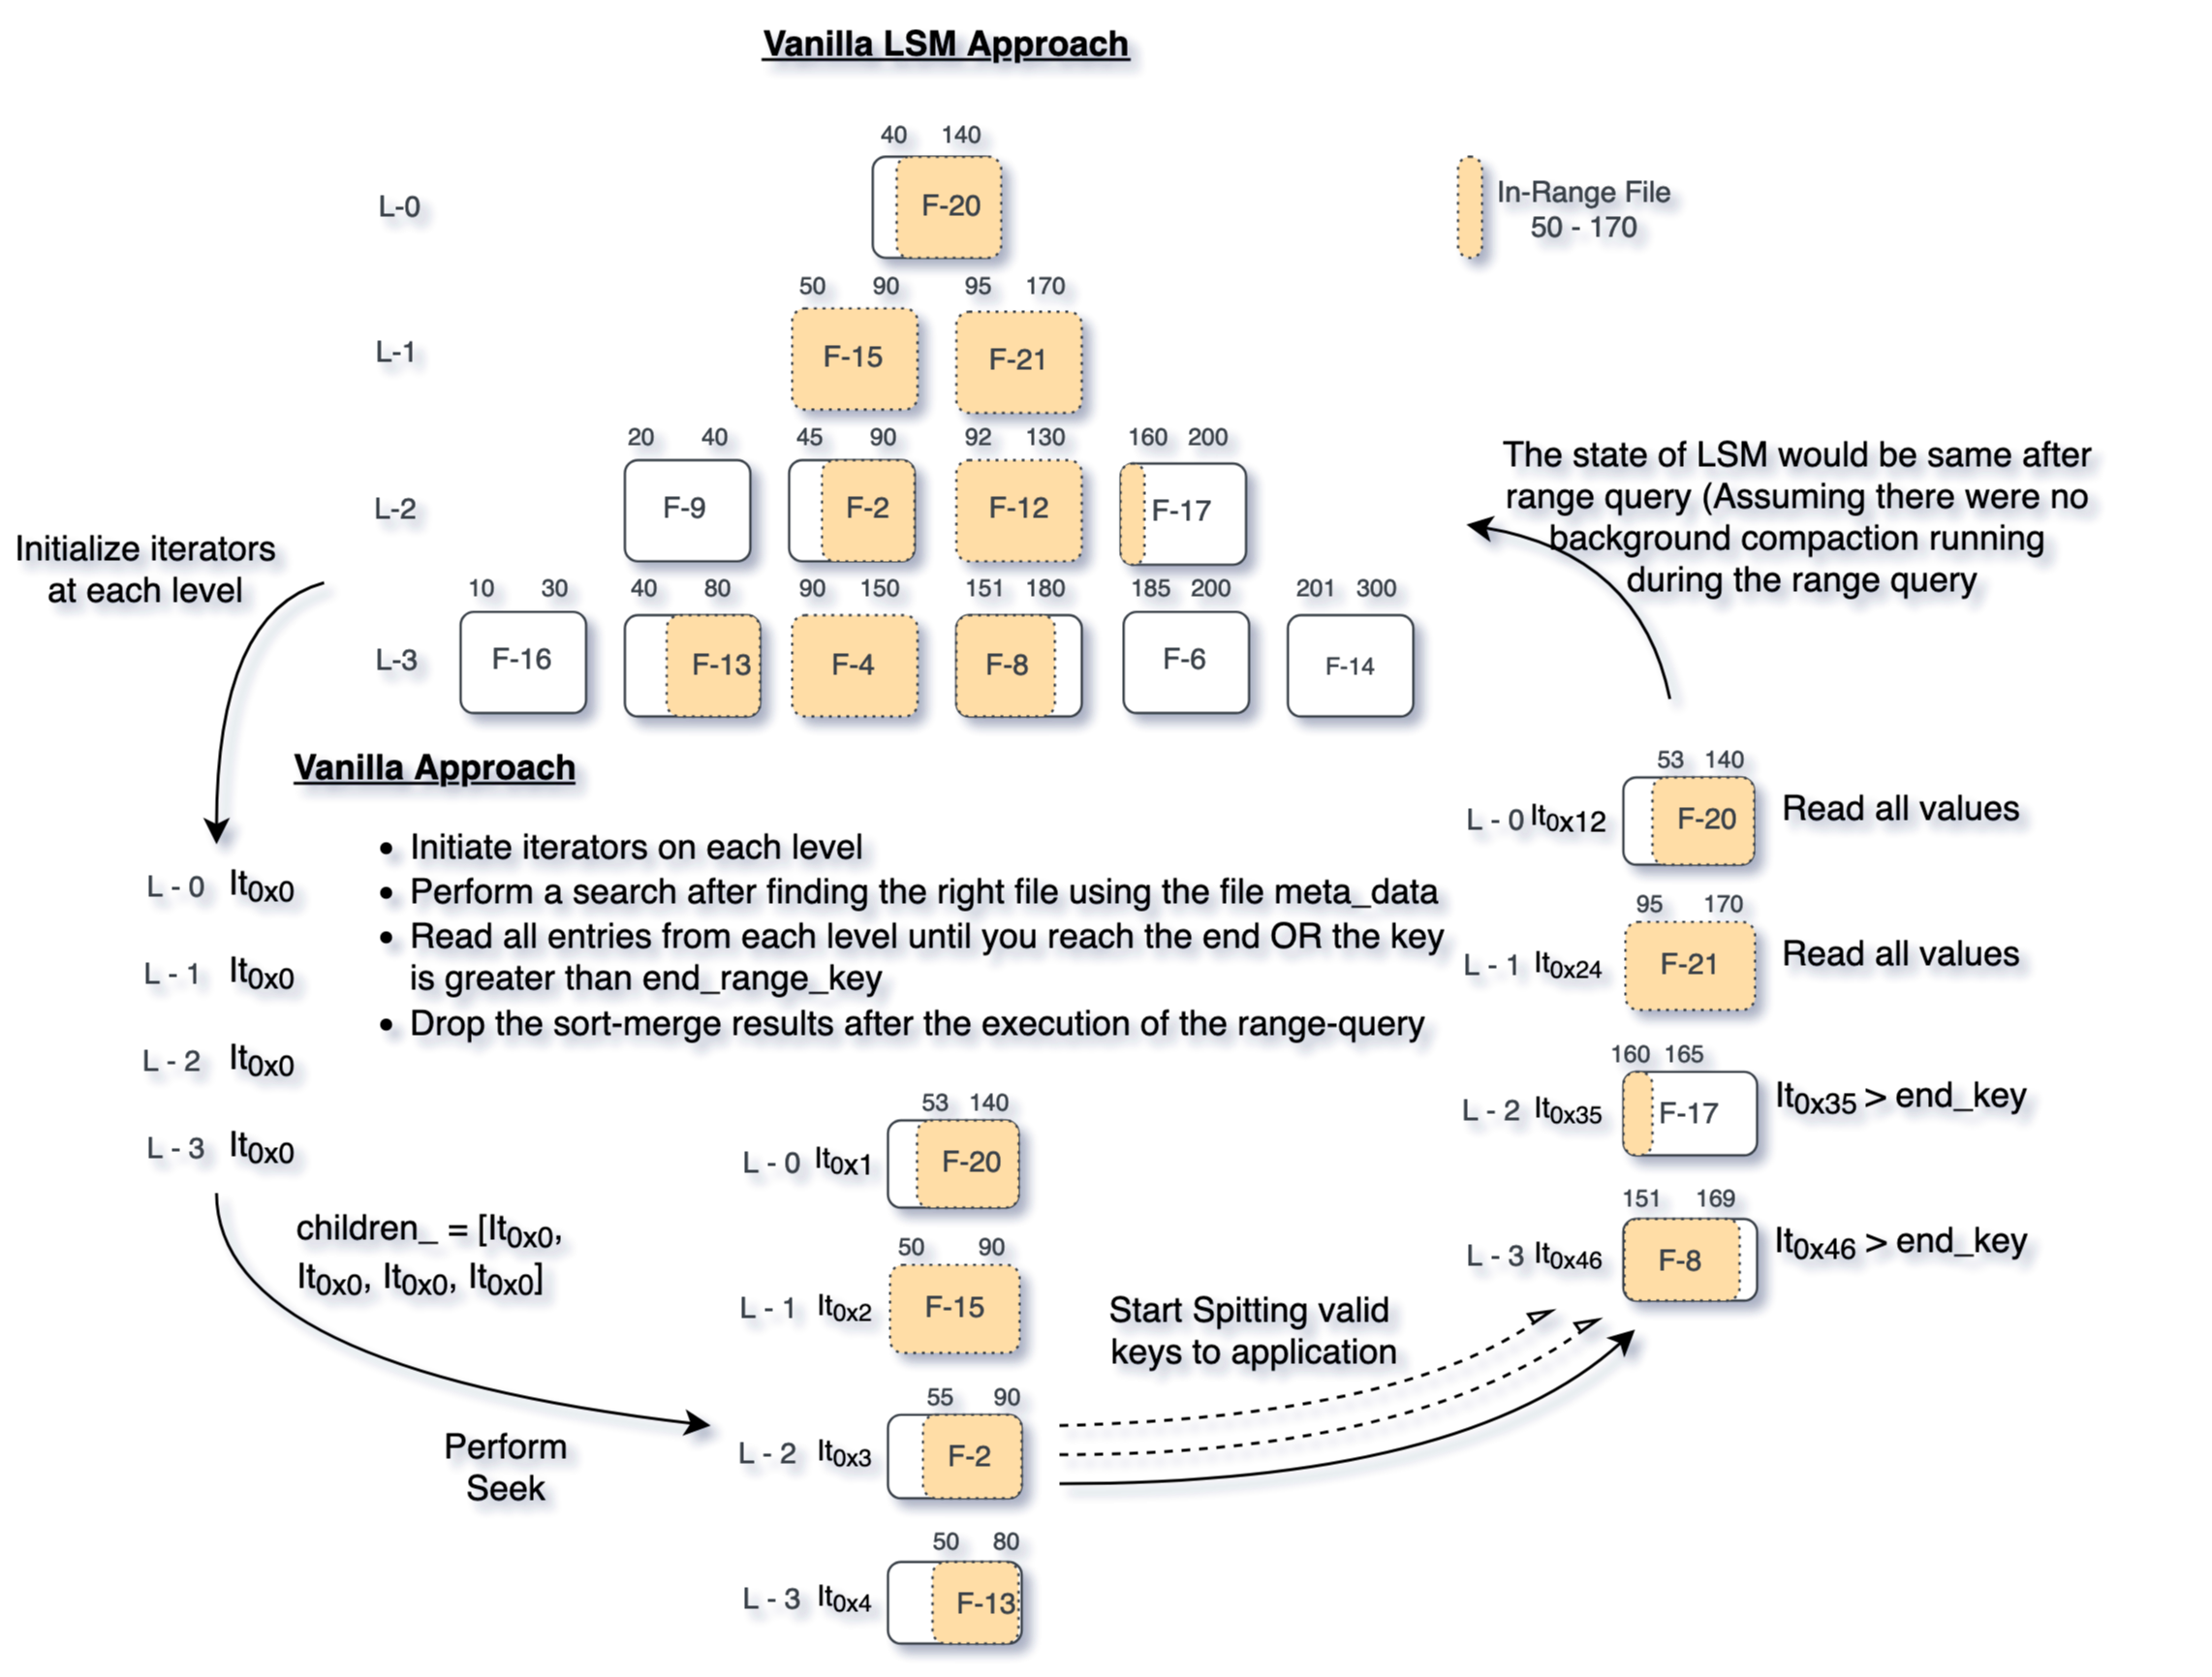
\includegraphics[scale=0.11]{Figures/Vanilla Range Query vanilla.png}
    \caption{Flow of ``vanilla'' range query in LSM. This outlines the sequential steps involved in a range 
    query}\label{fig:vanilla_range_query}
\end{figure}

\Paragraph{Improved Range Query Performance}
RQDC significantly enhances the efficiency of range queries, as evidenced by findings from a workload scenario same as 
above. In the vanilla approach, there was a continuous increase in the 
percentage of invalid keys read by range queries (shown in Figure~\ref{fig:increased_invalid_keys}), reaching up to 2\% of unique inserts by the end of the workload run. 
However, when the experiment was conducted with RQDC, specifically with lower and upper bounds set at 0 and 6, 
respectively, the percentage of invalid keys read by range queries came down to 0.7\% with a cost of a 30\% increase in 
average range query time (shown in Figure~\ref{fig:reduced_invalid_keys} and Figure~\ref{fig:increased_range_queries_time}). 
While there was a maximum spike of 0.7\% in the invalid keys read by 4 out of 100 range 
queries, the remaining 96\% of range queries read less than 0.5\% of invalid keys. We ran the same experiment with the 
lower and upper bound set to 0.25 and 1.5 with RQDC, showing a 1.1\% of invalid keys at the end of the experiment, 
which is lower than vanilla at a cost of a 2\% increase in average range query time (shown in Figure~\ref{fig:another_epoch_with_lb_ub} and Figure\ref{fig:range_queries_time}).

\Paragraph{Optimized Write Amplification}
While RQDC introduces additional writes during the query-driven compaction process, it maintains a competitive write 
amplification level similar to the vanilla approach using configurable lower bound and upper bound thresholds. The 
experiments that we ran for the same epoch workload showed that for the lower and upper bound of 0 and 6, the 
write amplification increases up to 5\% compared to vanilla, and for the lower and upper bound of 0.25 and 1.5, it
goes to 8\%. The strategy of eliminating invalid keys during compactions, triggered by range queries, increases write 
amplification slightly, which can be controlled by changing the values of the lower and upper bound.
